\documentclass[10pt]{beamer}
\usetheme{metropolis}

% ── Packages ──
\usepackage{amsmath,amssymb,amsthm}
\usepackage{tikz}
\usetikzlibrary{positioning,arrows.meta,fit,matrix,backgrounds,calc}
\usepackage{graphicx}
\usepackage{array}

% ── Theorem environments ──
\theoremstyle{definition}
\newtheorem{defi}{Definition}[section]
\newtheorem{prop}{Proposition}[section]
\newtheorem{thm}{Theorem}[section]
\newtheorem{cor}{Corollary}[section]

% ── Highlighting ──
\newcommand{\x}[1]{\alert{\textbf{#1}}}

\title{Lecture 5: Solving Linear Equations via Cross-Filling}
\subtitle{MATH203 Applied Linear Algebra}
\date{}

\begin{document}
\maketitle

% ═══════════════════════════════════════
% §1 MOTIVATION
% ═══════════════════════════════════════
\section{Motivation}

\begin{frame}{Today's Goal}

\x{Learn to solve}: $A\mathbf{x} = \mathbf{b}$ using the cross-filling method.

\vspace{1em}

\x{Why?}
\begin{itemize}
\item Find all solutions (existence)
\item Determine uniqueness
\item Find basis for null space (relationships between columns)
\end{itemize}

\vspace{1em}

\x{Method}: Decompose augmented matrix $(A \mid \mathbf{b})$ into rank-one pieces, extract simplified equations, solve backwards.

\end{frame}

% ═══════════════════════════════════════
% §2 COMPLETE EXAMPLE
% ═══════════════════════════════════════
\section{Complete Example: Solving $A\mathbf{x} = \mathbf{b}$}

\begin{frame}{Example Setup}

Solve:
$$A\mathbf{x} = \mathbf{b}$$

where

$$A = \begin{pmatrix}
1 & 2 & 1 \\
2 & 4 & 1 \\
3 & 6 & 2
\end{pmatrix}, \quad \mathbf{b} = \begin{pmatrix} 4 \\ 9 \\ 13 \end{pmatrix}$$

\vspace{1em}

\x{Strategy}: Form augmented matrix $(A \mid \mathbf{b})$, use cross-filling to simplify, then solve backwards.

\end{frame}

\begin{frame}{Original Equation System}

The matrix equation $A\mathbf{x} = \mathbf{b}$ represents three equations:

\vspace{0.5em}

\begin{align*}
\text{eq1}: \quad &x_1 + 2x_2 + x_3 = 4 \\
\text{eq2}: \quad &2x_1 + 4x_2 + x_3 = 9 \\
\text{eq3}: \quad &3x_1 + 6x_2 + 2x_3 = 13
\end{align*}

\vspace{1em}

\x{Goal}: Use cross-filling to transform this into a simpler equivalent system.

\end{frame}

\begin{frame}[fragile]{Step 1: Form Augmented Matrix}

\begin{center}
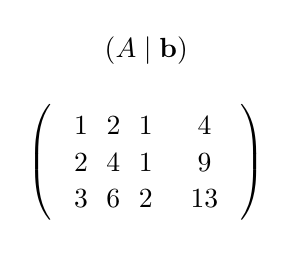
\begin{tikzpicture}[scale=0.8]
\matrix (m) [matrix of math nodes, left delimiter=(, right delimiter=), ampersand replacement=\&] {
1 \& 2 \& 1 \& \vrule \& 4 \\
2 \& 4 \& 1 \& \vrule \& 9 \\
3 \& 6 \& 2 \& \vrule \& 13 \\
};
\node[above=0.3cm of m] {$(A \mid \mathbf{b})$};
\end{tikzpicture}
\end{center}

\vspace{1em}

Each row represents one equation from our system.

\vspace{1em}

\x{Next}: Choose a pivot to begin cross-filling.

\end{frame}

\begin{frame}[fragile]{Step 2: Choose First Pivot at (1,1)}

\begin{center}
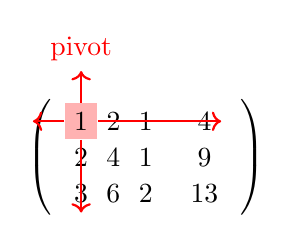
\begin{tikzpicture}[scale=0.8]
\matrix (m) [matrix of math nodes, left delimiter=(, right delimiter=), ampersand replacement=\&] {
|[fill=red!30]| 1 \& 2 \& 1 \& \vrule \& 4 \\
2 \& 4 \& 1 \& \vrule \& 9 \\
3 \& 6 \& 2 \& \vrule \& 13 \\
};
\draw[red, thick, ->] (m-1-1.north) -- ++(0, 0.5) node[above] {pivot};
\draw[red, thick, ->] (m-1-1.west) -- ++(-0.5, 0);
\draw[red, thick, ->] (m-1-1.east) -- (m-1-5.east);
\draw[red, thick, ->] (m-1-1.south) -- (m-3-1.south);
\end{tikzpicture}
\end{center}

\vspace{0.5em}

Pivot: entry $(1,1) = 1$ (red)

\vspace{0.5em}

\x{Cross-filling formula}:
$$(R_1 \mid \mathbf{b}_1) = \underbrace{\frac{\text{column 1}}{1}}_{\text{normalized column}} \cdot (\text{row 1})$$

\end{frame}

\begin{frame}[fragile]{Step 3: First Decomposition Result}

$$\underbrace{\begin{pmatrix}
1 & 2 & 1 & | & 4 \\
2 & 4 & 1 & | & 9 \\
3 & 6 & 2 & | & 13
\end{pmatrix}}_{(A \mid \mathbf{b})} = \underbrace{\begin{pmatrix}
\colorbox{red!20}{1} & \colorbox{red!20}{2} & \colorbox{red!20}{1} & | & \colorbox{red!20}{4} \\
\colorbox{red!20}{2} & \colorbox{red!20}{4} & \colorbox{red!20}{2} & | & \colorbox{red!20}{8} \\
\colorbox{red!20}{3} & \colorbox{red!20}{6} & \colorbox{red!20}{3} & | & \colorbox{red!20}{12}
\end{pmatrix}}_{(R_1 \mid \mathbf{b}_1) \text{ rank-one}} + \underbrace{\begin{pmatrix}
\alert{0} & 0 & 0 & | & \alert{0} \\
\alert{0} & 0 & -1 & | & 1 \\
\alert{0} & 0 & -1 & | & 1
\end{pmatrix}}_{\text{Remainder}}$$

\vspace{0.5em}

\x{Cross eliminates} (pivot at column 1, row 1):
\begin{itemize}
\item \alert{Column 1} eliminated in Remainder (pivot column)
\item \alert{Row 1} eliminated in Remainder (pivot row)
\item Column 2 remains 0 (free variable, unaffected by this cross)
\end{itemize}

\end{frame}

\begin{frame}{Step 5: Equations from $(R_1 \mid \mathbf{b}_1)$}

\x{The matrix}:
$$(R_1 \mid \mathbf{b}_1) = \begin{pmatrix}
1 & 2 & 1 & | & 4 \\
2 & 4 & 2 & | & 8 \\
3 & 6 & 3 & | & 12
\end{pmatrix}$$

\vspace{0.5em}

\x{Each row represents an equation}:
\begin{align*}
\text{Row 1}: &\quad 1x_1 + 2x_2 + 1x_3 = 4 \quad \text{(\x{eq1})} \\
\text{Row 2}: &\quad 2x_1 + 4x_2 + 2x_3 = 8 \quad \text{(\x{2·eq1})} \\
\text{Row 3}: &\quad 3x_1 + 6x_2 + 3x_3 = 12 \quad \text{(\x{3·eq1})}
\end{align*}

\x{Key}: All rows = same equation (eq1). Only \x{one independent equation}!

\end{frame}

\begin{frame}{Step 4: Understanding $(R_1 \mid \mathbf{b}_1)$}

\x{How did we get $(R_1 \mid \mathbf{b}_1)$?}

$$(R_1 \mid \mathbf{b}_1) = \begin{pmatrix} 1 \\ 2 \\ 3 \end{pmatrix} \begin{pmatrix} 1 & 2 & 1 & | & 4 \end{pmatrix}$$

\vspace{1em}

This is a \x{rank-one matrix}: all rows are multiples of row 1.

\end{frame}

\begin{frame}{Step 6: Equations from Remainder}

\x{The matrix}:
$$\text{Remainder} = \begin{pmatrix}
0 & 0 & 0 & | & 0 \\
0 & 0 & -1 & | & 1 \\
0 & 0 & -1 & | & 1
\end{pmatrix}$$

\vspace{0.5em}

\x{Each row represents an equation}:
\begin{align*}
\text{Row 1}: &\quad 0 = 0 \quad \text{(\alert{actively} zero: pivot row)} \\
\text{Row 2}: &\quad -x_3 = 1 \quad \text{(\alert{passively} zero in col 1: eq2 - 2·eq1)} \\
\text{Row 3}: &\quad -x_3 = 1 \quad \text{(\alert{passively} zero in col 1: eq3 - 3·eq1)}
\end{align*}

\x{Key distinction}:
\begin{itemize}
\item Row 1: \alert{actively} became zero (we chose it as pivot row)
\item Rows 2, 3: \alert{passively} became zero in column 1 (cross-filling eliminated it)
\end{itemize}

\end{frame}

\begin{frame}{Step 7: Understanding the Decomposition}

We decomposed $(A \mid \mathbf{b}) = (R_1 \mid \mathbf{b}_1) + \text{Remainder}$:

\vspace{1em}

\begin{center}
\begin{tabular}{c|c|c}
\textbf{Matrix} & \textbf{Equations contained} & \textbf{Relation to original} \\
\hline
$(R_1 \mid \mathbf{b}_1)$ & eq1 (×3 rows) & eq1 \\
\hline
Remainder & $-x_3 = 1$ (×2 rows) & eq2 $-$ 2·eq1, eq3 $-$ 3·eq1 \\
\end{tabular}
\end{center}

\vspace{1em}

\x{Simplified equation system}:
\begin{align*}
\text{From } R_1: \quad &x_1 + 2x_2 + x_3 = 4 \\
\text{From Remainder}: \quad &x_3 = -1
\end{align*}

\vspace{0.5em}

This is equivalent to the original three equations!

\end{frame}

\begin{frame}[fragile]{Step 8: Continue Cross-Filling on Remainder}

The Remainder still has structure. Choose second pivot at $(2,3) = -1$:

\begin{center}
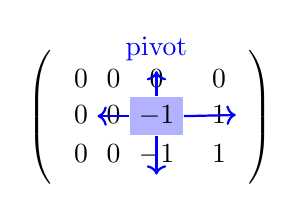
\begin{tikzpicture}[scale=0.8]
\matrix (m) [matrix of math nodes, left delimiter=(, right delimiter=), ampersand replacement=\&] {
0 \& 0 \& 0 \& \vrule \& 0 \\
0 \& 0 \& |[fill=blue!30]| -1 \& \vrule \& 1 \\
0 \& 0 \& -1 \& \vrule \& 1 \\
};
\draw[blue, thick, ->] (m-2-3.north) -- ++(0, 0.4) node[above] {pivot};
\draw[blue, thick, ->] (m-2-3.west) -- ++(-0.5, 0);
\draw[blue, thick, ->] (m-2-3.east) -- (m-2-5.east);
\draw[blue, thick, ->] (m-2-3.south) -- (m-3-3.south);
\end{tikzpicture}
\end{center}

\vspace{0.5em}

$$(R_2 \mid \mathbf{b}_2) = \frac{\text{column 3 of Remainder}}{-1} \cdot (\text{row 2 of Remainder})$$

\end{frame}

\begin{frame}[fragile]{Step 9: Second Decomposition Result}

$$\underbrace{\begin{pmatrix}
0 & 0 & \alert{0} & | & \alert{0} \\
\alert{0} & \alert{0} & \alert{-1} & | & \alert{1} \\
0 & 0 & \alert{-1} & | & \alert{1}
\end{pmatrix}}_{\text{First Remainder}} = \underbrace{\begin{pmatrix}
\colorbox{blue!20}{0} & \colorbox{blue!20}{0} & \colorbox{blue!20}{0} & | & \colorbox{blue!20}{0} \\
\colorbox{blue!20}{0} & \colorbox{blue!20}{0} & \colorbox{blue!20}{1} & | & \colorbox{blue!20}{-1} \\
\colorbox{blue!20}{0} & \colorbox{blue!20}{0} & \colorbox{blue!20}{1} & | & \colorbox{blue!20}{-1}
\end{pmatrix}}_{(R_2 \mid \mathbf{b}_2) \text{ rank-one}} + \underbrace{\begin{pmatrix}
0 & 0 & \alert{0} & | & \alert{0} \\
\alert{0} & \alert{0} & \alert{0} & | & \alert{0} \\
0 & 0 & \alert{0} & | & \alert{0}
\end{pmatrix}}_{\text{All zeros!}}$$

\vspace{1em}

\x{Cross-filling complete}: $(A \mid \mathbf{b}) = (R_1 \mid \mathbf{b}_1) + (R_2 \mid \mathbf{b}_2)$

\end{frame}

\begin{frame}{Step 10: Equations from $(R_2 \mid \mathbf{b}_2)$}

\x{The matrix}:
$$(R_2 \mid \mathbf{b}_2) = \begin{pmatrix}
0 & 0 & 0 & | & 0 \\
0 & 0 & 1 & | & -1 \\
0 & 0 & 1 & | & -1
\end{pmatrix}$$

\vspace{0.5em}

\x{Each row represents an equation}:
\begin{align*}
\text{Row 1}: &\quad 0 = 0 \quad \text{(inherited zero from Remainder)} \\
\text{Row 2}: &\quad x_3 = -1 \quad \text{(\alert{actively} extracted: pivot row)} \\
\text{Row 3}: &\quad x_3 = -1 \quad \text{(\alert{passively} copied: non-pivot row)}
\end{align*}

\x{Note}: Row 2 was chosen as pivot row; row 3 passively gets the same equation.

\end{frame}

\begin{frame}{Step 10 (continued): Final Remainder Analysis}

After extracting $(R_2 \mid \mathbf{b}_2)$, the final Remainder is all zeros:

$$\text{Final Remainder} = \begin{pmatrix}
0 & 0 & 0 & | & 0 \\
0 & 0 & 0 & | & 0 \\
0 & 0 & 0 & | & 0
\end{pmatrix}$$

\x{How did each row become zero?}
\begin{itemize}
\item Row 1: was already 0 (inherited)
\item Row 2: \alert{actively} became 0 (we chose it as pivot row)
\item Row 3: \alert{passively} became 0 (row 3 - row 2, column 3 eliminated)
\end{itemize}

\x{Cross-filling complete!}

\end{frame}

\begin{frame}{Step 11: The Simplified Equation System}

From the cross-filling decomposition, we extracted:

\vspace{1em}

\begin{center}
\begin{tabular}{c|l}
\textbf{From piece} & \textbf{Equation} \\
\hline
$(R_1 \mid \mathbf{b}_1)$ & $\alert{x_1} + 2x_2 + \alert{x_3} = 4$ \\
& (pivot: $\alert{x_1}$, free: $x_2$, $\alert{x_3}$ not yet determined) \\
\hline
$(R_2 \mid \mathbf{b}_2)$ & $\alert{x_3} = -1$ \\
& (pivot: $\alert{x_3}$) \\
\end{tabular}
\end{center}

\vspace{1em}

\x{Variable classification} (from cross-filling):
\begin{itemize}
\item \x{Pivot variables}: $x_1, x_3$ (columns 1 and 3 where we chose pivots)
\item \x{Free variable}: $x_2$ (column 2, non-pivot column)
\end{itemize}

\end{frame}

\begin{frame}{Step 12: Backward Solving}

Solve from the \x{simplest equation} backwards:

\vspace{1em}

\x{From equation 2}:
$$x_3 = -1$$

\vspace{1em}

\x{Substitute into equation 1}:
\begin{align*}
x_1 + 2x_2 + x_3 &= 4 \\
x_1 + 2x_2 + (-1) &= 4 \\
x_1 + 2x_2 &= 5 \\
x_1 &= 5 - 2x_2
\end{align*}

\vspace{1em}

\x{Variable $x_2$ is not determined} by any equation!

\end{frame}

\begin{frame}{Step 13: Identify Pivot and Free Variables}

From cross-filling, we chose pivots at:
\begin{itemize}
\item Column 1 (first pivot)
\item Column 3 (second pivot)
\end{itemize}

\vspace{1em}

\x{Classification}:
\begin{itemize}
\item \x{Pivot variables}: $x_1, x_3$ (determined by equations)
\item \x{Free variable}: $x_2$ (can be chosen freely)
\end{itemize}

\vspace{1em}

\x{Pivot columns} = columns where we chose pivots.

\x{Non-pivot columns} = remaining columns $\to$ free variables.

\end{frame}

\begin{frame}{Step 14: General Solution}

Let $x_2 = t$ (free parameter).

\vspace{1em}

From our backward solving:
\begin{align*}
x_1 &= 5 - 2t \\
x_2 &= t \\
x_3 &= -1
\end{align*}

\vspace{1em}

\x{General solution}:
$$\mathbf{x} = \begin{pmatrix} 5 - 2t \\ t \\ -1 \end{pmatrix}$$

\vspace{1em}

This describes \x{infinitely many solutions} (one for each value of $t$).

\end{frame}

\begin{frame}{Step 15: Decompose into Particular + Null Space}

Rewrite the general solution:

$$\mathbf{x} = \begin{pmatrix} 5 - 2t \\ t \\ -1 \end{pmatrix} = \begin{pmatrix} 5 \\ 0 \\ -1 \end{pmatrix} + t \begin{pmatrix} -2 \\ 1 \\ 0 \end{pmatrix}$$

\vspace{1em}

\x{Two parts}:
\begin{itemize}
\item \x{Particular solution} $\mathbf{x}_p = \begin{pmatrix} 5 \\ 0 \\ -1 \end{pmatrix}$ (when $t=0$)
\item \x{Null space direction} $\mathbf{v} = \begin{pmatrix} -2 \\ 1 \\ 0 \end{pmatrix}$ (coefficient of $t$)
\end{itemize}

\vspace{1em}

Check: $A\mathbf{v} = \mathbf{0}$ (verify this is in null space).

\end{frame}

\begin{frame}{Step 16: Verification (Particular Solution)}

\x{Verify particular solution}: $A\mathbf{x}_p = \mathbf{b}$

$$\begin{pmatrix} 1&2&1 \\ 2&4&1 \\ 3&6&2 \end{pmatrix} \begin{pmatrix} 5\\0\\-1 \end{pmatrix} = \begin{pmatrix} 5+0-1 \\ 10+0-1 \\ 15+0-2 \end{pmatrix} = \begin{pmatrix} 4\\9\\13 \end{pmatrix}$$ \checkmark

\end{frame}

\begin{frame}{Step 16: Verification (Null Space Vector) (continued)}

\x{Verify null space vector}: $A\mathbf{v} = \mathbf{0}$

$$\begin{pmatrix} 1&2&1 \\ 2&4&1 \\ 3&6&2 \end{pmatrix} \begin{pmatrix} -2\\1\\0 \end{pmatrix} = \begin{pmatrix} -2+2+0 \\ -4+4+0 \\ -6+6+0 \end{pmatrix} = \begin{pmatrix} 0\\0\\0 \end{pmatrix}$$ \checkmark

\vspace{1em}

Both parts of the solution are verified!

\end{frame}

\begin{frame}{Summary of the Example}

\x{What we did}:
\begin{enumerate}
\item Formed augmented matrix $(A \mid \mathbf{b})$
\item Used cross-filling to decompose into rank-one pieces
\item Extracted simplified equations from each piece
\item Solved backwards from simplest equation
\item Identified free variables
\item Wrote general solution = particular + null space
\end{enumerate}

\vspace{1em}

\x{Key insight}: Cross-filling transforms the original equation system into an \textbf{equivalent simpler system} where variables decrease step-by-step.

\end{frame}

% ═══════════════════════════════════════
% §3 WHY VARIABLES DECREASE
% ═══════════════════════════════════════
\section{Why Variables Decrease}

\begin{frame}{Observation: Variables Decrease with Each Piece}

In our example:

\vspace{1em}

\begin{center}
\begin{tabular}{c|c|c}
\textbf{Piece} & \textbf{Active variables} & \textbf{Count} \\
\hline
Original $(A \mid \mathbf{b})$ & $x_1, x_2, x_3$ & 3 \\
\hline
After extracting $R_1$ & & \\
Remainder & $x_3$ only & 1 \\
\hline
After extracting $R_2$ & & \\
Final Remainder & none & 0 \\
\end{tabular}
\end{center}

\vspace{1em}

\x{Pattern}: Each cross-filling step eliminates at least one variable from the remainder.

\end{frame}

\begin{frame}{Why Does This Happen?}

\x{Cross-filling structure}:

$$(R_i \mid \mathbf{b}_i) = \frac{\text{column } j}{a_{kj}} \cdot (\text{row } k)$$

\vspace{1em}

\begin{itemize}
\item All rows of $(R_i \mid \mathbf{b}_i)$ are multiples of row $k$
\item When we subtract $(R_i \mid \mathbf{b}_i)$ from the matrix, column $j$ becomes zero in the remainder
\item Column $j$ is \x{eliminated} from future consideration
\end{itemize}

\vspace{1em}

\x{Result}: Each step reduces the number of active columns (variables) by at least one.

\end{frame}

\begin{frame}{Consequence: Backward Solving Works}

Since variables decrease:

\vspace{1em}

\begin{itemize}
\item Last piece $(R_r \mid \mathbf{b}_r)$ has \x{fewest variables}
\item Second-to-last has one more variable
\item $\vdots$
\item First piece has most variables
\end{itemize}

\vspace{1em}

\x{Backward solving strategy}:
\begin{enumerate}
\item Start from the last equation (fewest variables)
\item Solve for pivot variable(s)
\item Substitute into previous equation
\item Repeat until all pivot variables determined
\end{enumerate}

\end{frame}

% ═══════════════════════════════════════
% §4 EXISTENCE AND UNIQUENESS
% ═══════════════════════════════════════
\section{Existence and Uniqueness}

\begin{frame}{When Does $A\mathbf{x} = \mathbf{b}$ Have a Solution?}

\x{Key question}: After cross-filling $(A \mid \mathbf{b})$, what determines existence of solutions?

\vspace{1em}

\x{Strategy}: Always choose pivots \textbf{inside $A$} (not in $\mathbf{b}$ column).

\vspace{1em}

\x{Two possible outcomes}:
\begin{enumerate}
\item \textbf{$\mathbf{b}$ column clears to zero} $\Rightarrow$ solution exists
\item \textbf{$\mathbf{b}$ column has residue after $A$ clears} $\Rightarrow$ no solution
\end{enumerate}

\vspace{1em}

Let's see a concrete \x{no-solution example}$\ldots$

\end{frame}

% ═══ DETAILED NO-SOLUTION EXAMPLE ═══
\begin{frame}{Example: A System with NO Solution}

Same $A$ matrix, but \alert{different $\mathbf{b}$}:

$$A = \begin{pmatrix}
1 & 2 & 1 \\
2 & 4 & 1 \\
3 & 6 & 2
\end{pmatrix}, \quad \mathbf{b} = \begin{pmatrix} 4 \\ 9 \\ \alert{14} \end{pmatrix}$$

\vspace{0.5em}

\x{Note}: Changed last entry from 13 to \alert{14}.

\vspace{1em}

\x{Question}: Can we solve $A\mathbf{x} = \mathbf{b}$?

\vspace{0.5em}

\x{Method}: Cross-fill $(A \mid \mathbf{b})$ with pivots \textbf{only in $A$'s columns}.

\end{frame}

\begin{frame}[fragile]{No-Solution Example: Initial Augmented Matrix}

$$(A \mid \mathbf{b}) = \begin{pmatrix}
1 & 2 & 1 & | & 4 \\
2 & 4 & 1 & | & 9 \\
3 & 6 & 2 & | & \alert{14}
\end{pmatrix}$$

\vspace{1em}

\x{Cross-filling rule}: Choose pivots \textbf{only in columns 1, 2, 3} (inside $A$).

\vspace{1em}

\x{Number of cross-fillings we can do on $A$} = rank$(A)$.

\vspace{0.5em}

For this $A$: rank$(A) = 2$ (we'll see this as we go).

\end{frame}

\begin{frame}[fragile]{No-Solution Step 1: First Cross-Filling}

Choose pivot at (1,1):

$$\underbrace{\begin{pmatrix}
1 & 2 & 1 & | & 4 \\
2 & 4 & 1 & | & 9 \\
3 & 6 & 2 & | & \alert{14}
\end{pmatrix}}_{(A \mid \mathbf{b})} = \underbrace{\begin{pmatrix}
\colorbox{red!20}{1} & \colorbox{red!20}{2} & \colorbox{red!20}{1} & | & \colorbox{red!20}{4} \\
\colorbox{red!20}{2} & \colorbox{red!20}{4} & \colorbox{red!20}{2} & | & \colorbox{red!20}{8} \\
\colorbox{red!20}{3} & \colorbox{red!20}{6} & \colorbox{red!20}{3} & | & \colorbox{red!20}{12}
\end{pmatrix}}_{(R_1 \mid \mathbf{b}_1)} + \underbrace{\begin{pmatrix}
\alert{0} & 0 & 0 & | & \alert{0} \\
\alert{0} & 0 & -1 & | & 1 \\
\alert{0} & 0 & -1 & | & \alert{2}
\end{pmatrix}}_{\text{Remainder}}$$

\vspace{0.5em}

\x{Cross eliminates} (pivot at column 1, row 1):
\begin{itemize}
\item \alert{Column 1} eliminated: entries $(2,1)$ and $(3,1)$ become 0
\item \alert{Row 1} eliminated: entire row 1 becomes 0
\item Column 2 remains 0 (free variable column, not affected by this cross)
\item \alert{$\mathbf{b}$ column changed}: $14 \to 12 + \alert{2}$ residue
\end{itemize}

\end{frame}

\begin{frame}[fragile]{No-Solution Step 2: Second Cross-Filling}

Choose pivot at (2,3) in Remainder:

$$\underbrace{\begin{pmatrix}
0 & 0 & \alert{0} & | & \alert{0} \\
\alert{0} & \alert{0} & \alert{-1} & | & \alert{1} \\
0 & 0 & \alert{-1} & | & \alert{2}
\end{pmatrix}}_{\text{First Remainder}} = \underbrace{\begin{pmatrix}
\colorbox{blue!20}{0} & \colorbox{blue!20}{0} & \colorbox{blue!20}{0} & | & \colorbox{blue!20}{0} \\
\colorbox{blue!20}{0} & \colorbox{blue!20}{0} & \colorbox{blue!20}{1} & | & \colorbox{blue!20}{-1} \\
\colorbox{blue!20}{0} & \colorbox{blue!20}{0} & \colorbox{blue!20}{1} & | & \colorbox{blue!20}{-1}
\end{pmatrix}}_{(R_2 \mid \mathbf{b}_2)} + \underbrace{\begin{pmatrix}
0 & 0 & \alert{0} & | & \alert{0} \\
\alert{0} & \alert{0} & \alert{0} & | & \alert{0} \\
0 & 0 & \alert{0} & | & \alert{\boxed{1}}
\end{pmatrix}}_{\text{Second Remainder}}$$

\vspace{0.5em}

\x{Cross eliminates} (pivot at column 3, row 2):
\begin{itemize}
\item \alert{Column 3} eliminated: entries $(1,3)$ and $(3,3)$ become 0
\item \alert{Row 2} eliminated: entire row 2 becomes 0
\item Column 1 already 0 (from previous cross), column 2 still 0 (free variable)
\item \alert{$\mathbf{b}$ column residue}: $\boxed{1} \neq 0$ remains!
\end{itemize}

\end{frame}

\begin{frame}{No-Solution: Why Residue Means No Solution}

Second Remainder row 3:
$$\begin{pmatrix} \alert{0} & \alert{0} & \alert{0} & | & \alert{\boxed{1}} \end{pmatrix}$$

\vspace{1em}

\x{This represents the equation}:
$$0 \cdot x_1 + 0 \cdot x_2 + 0 \cdot x_3 = 1$$
$$\Downarrow$$
$$0 = 1 \quad \text{(\alert{CONTRADICTION!})}$$

\vspace{1em}

\x{Why did this happen?}
\begin{itemize}
\item We exhausted all pivots in $A$ (rank$(A) = 2$, did 2 cross-fillings)
\item $A$ part completely cleared
\item But $\mathbf{b}$ column still has residue (1 left over)
\item \alert{This means $\mathbf{b} \notin \text{Col}(A)$}
\end{itemize}

\end{frame}

\begin{frame}{No-Solution: Cannot Fix by More Cross-Filling}

\x{Can we do another cross-filling to clear the residue?}

\vspace{1em}

Second Remainder:
$$\begin{pmatrix}
\alert{0} & \alert{0} & \alert{0} & | & \alert{0} \\
\alert{0} & \alert{0} & \alert{0} & | & \alert{0} \\
\alert{0} & \alert{0} & \alert{0} & | & \alert{\boxed{1}}
\end{pmatrix}$$

\vspace{1em}

\x{Problem}: The only non-zero entry is in the $\mathbf{b}$ column!

\vspace{1em}

If we choose pivot at (3,4) (in $\mathbf{b}$ column):
$$(R_3 \mid \mathbf{b}_3) = \begin{pmatrix} 0 \\ 0 \\ 1 \end{pmatrix} \begin{pmatrix} 0 & 0 & 0 & | & 1 \end{pmatrix} = \begin{pmatrix}
0 & 0 & 0 & | & 0 \\
0 & 0 & 0 & | & 0 \\
0 & 0 & 0 & | & 1
\end{pmatrix}$$

Still gives equation $0 = 1$! \alert{Cannot avoid contradiction.}

\end{frame}

\begin{frame}{No-Solution: The Key Insight}

\x{Rank interpretation}:
\begin{itemize}
\item rank$(A) = 2$: We can do \textbf{2 cross-fillings} on $A$
\item After 2 cross-fillings, $A$ part is completely zero
\item If $\mathbf{b}$ column has residue, rank$(A \mid \mathbf{b}) = 3 > 2$
\item \alert{This extra "rank" forces a contradiction row}
\end{itemize}

\vspace{1em}

\x{General principle}:
\begin{center}
\fbox{\begin{minipage}{0.85\textwidth}
rank$(A \mid \mathbf{b}) > $ rank$(A)$ \\
$\Updownarrow$ \\
$\mathbf{b}$ has residue after $A$ clears \\
$\Updownarrow$ \\
Contradiction row $0 = c$ ($c \neq 0$) appears \\
$\Updownarrow$ \\
\textbf{No solution}
\end{minipage}}
\end{center}

\end{frame}

\begin{frame}{Existence Criterion}

\begin{thm}[Existence]
$A\mathbf{x} = \mathbf{b}$ has a solution if and only if:
$$\text{rank}(A \mid \mathbf{b}) = \text{rank}(A)$$
\end{thm}

\vspace{1em}

\x{Interpretation}:
\begin{itemize}
\item If adding $\mathbf{b}$ as a column doesn't increase rank $\Rightarrow$ $\mathbf{b}$ is already in the span of $A$'s columns
\item Equivalently: $\mathbf{b} \in \text{Col}(A)$
\end{itemize}

\end{frame}

\begin{frame}{Uniqueness Criterion}

If a solution exists, is it unique?

\vspace{1em}

\begin{thm}[Uniqueness]
If $A\mathbf{x} = \mathbf{b}$ has a solution, it is \x{unique} if and only if:
$$\text{Null}(A) = \{\mathbf{0}\}$$

Equivalently:
\begin{itemize}
\item No free variables
\item $\text{rank}(A) = n$ (number of columns)
\end{itemize}
\end{thm}

\vspace{1em}

\x{Proof idea}: If $\mathbf{x}_1, \mathbf{x}_2$ both solve $A\mathbf{x}=\mathbf{b}$, then $\mathbf{x}_1 - \mathbf{x}_2 \in \text{Null}(A)$.

\end{frame}

\begin{frame}{The Four Cases}

\begin{center}
\begin{tabular}{c|c|c}
& \textbf{rank}$(A) = n$ & \textbf{rank}$(A) < n$ \\
& (no free vars) & (has free vars) \\
\hline
\textbf{rank}$(A \mid \mathbf{b})$ & \x{Unique} & \x{Infinitely many} \\
$= $ \textbf{rank}$(A)$ & solution & solutions \\
(consistent) & & \\
\hline
\textbf{rank}$(A \mid \mathbf{b})$ & \x{No solution} & \x{No solution} \\
$= $ \textbf{rank}$(A) + 1$ & & \\
(inconsistent) & & \\
\end{tabular}
\end{center}

\vspace{1em}

Our example: rank$(A)=2$, rank$(A \mid \mathbf{b})=2$, $n=3$ $\Rightarrow$ infinitely many solutions.

\end{frame}

% ═══════════════════════════════════════
% §5 FINDING NULL SPACE BASIS
% ═══════════════════════════════════════
\section{Finding Null Space Basis}

\begin{frame}{Definition: Null Space}

\begin{defi}[Null Space]
For a matrix $A \in \mathbb{R}^{m \times n}$:
$$\text{Null}(A) = \{\mathbf{x} \in \mathbb{R}^n : A\mathbf{x} = \mathbf{0}\}$$
\end{defi}

\vspace{1em}

\x{Meaning}: Vectors that get mapped to zero.

\vspace{1em}

\x{Interpretation}: Relationships between the columns of $A$.

\vspace{1em}

If $\mathbf{v} \in \text{Null}(A)$, then $v_1 \mathbf{a}_1 + \cdots + v_n \mathbf{a}_n = \mathbf{0}$ (linear dependence).

\end{frame}

\begin{frame}{Example: Finding Null Space Basis for Our Matrix}

Solve $A\mathbf{x} = \mathbf{0}$:

$$A = \begin{pmatrix} 1&2&1 \\ 2&4&1 \\ 3&6&2 \end{pmatrix}$$

\vspace{1em}

Form $(A \mid \mathbf{0})$ and cross-fill (same steps as before, but with $\mathbf{b} = \mathbf{0}$):

\vspace{0.5em}

Simplified system:
\begin{align*}
x_1 + 2x_2 + x_3 &= 0 \\
x_3 &= 0
\end{align*}

\end{frame}

\begin{frame}{Backward Solving for Null Space}

From the simplified system:
\begin{align*}
x_3 &= 0 \\
x_1 + 2x_2 + 0 &= 0 \quad \Rightarrow \quad x_1 = -2x_2
\end{align*}

\vspace{1em}

Free variable: $x_2 = t$

\vspace{1em}

\x{General null space vector}:
$$\mathbf{x} = \begin{pmatrix} -2t \\ t \\ 0 \end{pmatrix} = t \begin{pmatrix} -2 \\ 1 \\ 0 \end{pmatrix}$$

\vspace{1em}

\x{Basis for Null}$(A)$: $\left\{ \begin{pmatrix} -2\\1\\0 \end{pmatrix} \right\}$

\end{frame}

\begin{frame}{General Procedure: Finding Null Space Basis}

\begin{prop}
To find a basis for $\text{Null}(A)$:
\begin{enumerate}
\item Solve $A\mathbf{x} = \mathbf{0}$ using cross-filling
\item Identify free variables (non-pivot columns)
\item For each free variable: set it to 1, others to 0, solve for pivots
\item Each setting gives one basis vector
\end{enumerate}
\end{prop}

\vspace{1em}

\x{Dimension of Null}$(A)$ = number of free variables.

\end{frame}

% ═══════════════════════════════════════
% §6 RANK-NULLITY THEOREM
% ═══════════════════════════════════════
\section{Rank-Nullity Theorem}

\begin{frame}{Counting Pivot and Free Variables}

For an $m \times n$ matrix $A$:

\vspace{1em}

\begin{itemize}
\item Total columns: $n$
\item Pivot columns (from cross-filling): $r = \text{rank}(A)$
\item Non-pivot columns (free variables): $n - r$
\end{itemize}

\vspace{1em}

But non-pivot columns = dimension of null space!

\vspace{1em}

$$\dim(\text{Null}(A)) = n - r$$

\end{frame}

\begin{frame}{Rank-Nullity Theorem}

\begin{thm}[Rank-Nullity Theorem]
For any $m \times n$ matrix $A$:
$$\boxed{\text{rank}(A) + \dim(\text{Null}(A)) = n}$$
\end{thm}

\vspace{1em}

\x{Proof}: Every column is either:
\begin{itemize}
\item A pivot column (contributes to rank), or
\item A non-pivot column (contributes one basis vector to null space)
\end{itemize}

These counts partition the $n$ columns.

\vspace{1em}

Also written: $\text{rank}(A) + \text{nullity}(A) = n$

\end{frame}

\begin{frame}{Example Verification}

Our $3 \times 3$ example:

$$A = \begin{pmatrix} 1&2&1 \\ 2&4&1 \\ 3&6&2 \end{pmatrix}$$

\vspace{1em}

\begin{itemize}
\item $n = 3$ (three columns)
\item rank$(A) = 2$ (two pivot columns: 1 and 3)
\item dim(Null$(A)$) = 1 (one free variable: $x_2$)
\end{itemize}

\vspace{1em}

Check: $2 + 1 = 3$ \checkmark

\end{frame}

% ═══════════════════════════════════════
% §7 SUMMARY
% ═══════════════════════════════════════
\section{Summary}

\begin{frame}{What We Learned}

\x{Cross-filling method for solving $A\mathbf{x} = \mathbf{b}$}:
\begin{enumerate}
\item Decompose $(A \mid \mathbf{b})$ into rank-one pieces
\item Each piece gives one simplified equation
\item Variables decrease with each piece
\item Solve backwards from simplest equation
\end{enumerate}

\vspace{1em}

\x{Key results}:
\begin{itemize}
\item Existence: rank$(A \mid \mathbf{b}) = $ rank$(A)$
\item Uniqueness: Null$(A) = \{\mathbf{0}\}$
\item General solution = particular + null space
\item Rank-Nullity: rank$(A) + $ nullity $ = n$
\end{itemize}

\end{frame}

\begin{frame}{Next Lecture}

\x{Lecture 6: Four Fundamental Subspaces}

\vspace{1em}

We'll explore:
\begin{itemize}
\item Column space and null space (from today)
\item Row space and left null space
\item Orthogonality relationships: Null$(A) \perp $ Row$(A)$
\item The fundamental theorem of linear algebra
\end{itemize}

\end{frame}

\end{document}
